\documentclass{scrreprt}
\usepackage{listings}
\usepackage{underscore}
\usepackage{graphicx}
\usepackage[bookmarks=true]{hyperref}
\usepackage[utf8]{inputenc}
\usepackage[english]{babel}
\usepackage{hyperref}
\usepackage{tabularx}
\usepackage{imakeidx}
\usepackage[colorinlistoftodos]{todonotes}
\makeindex[intoc]
\usepackage{graphicx}
\graphicspath{ {./Pictures/} }
\usepackage{ltablex}

\hypersetup{
    bookmarks=false,    % show bookmarks bar?
    pdftitle={Software Requirement Specification},    % title
    pdfauthor={Analysis Team},                     % author
    pdfsubject={TeX and LaTeX},                        % subject of the document
    pdfkeywords={TeX, LaTeX, graphics, images}, % list of keywords
    colorlinks=true,       % false: boxed links; true: colored links
    linkcolor=blue,       % color of internal links
    citecolor=black,       % color of links to bibliography
    filecolor=black,        % color of file links
    urlcolor=blue,        % color of external links
    linktoc=page            % only page is linked
}%
\def\myversion{2.4}
\title{Software Requirements Specification}
\author{Sara Lindholm \\ Patrick Asman \\ Jacob Rhan}

\date{October 2020}

\newcolumntype{s}{>{\hsize=3.75\hsize}X}
\newcolumntype{m}{>{\hsize=7\hsize}X}
\newcolumntype{b}{>{\hsize=11\hsize}X}

\makeatletter
\renewenvironment{thebibliography}[1]
     {\section{\bibname}% <-- this line was changed from \chapter* to \section*
      \@mkboth{\MakeUppercase\bibname}{\MakeUppercase\bibname}%
      \list{\@biblabel{\@arabic\c@enumiv}}%
           {\settowidth\labelwidth{\@biblabel{#1}}%
            \leftmargin\labelwidth
            \advance\leftmargin\labelsep
            \@openbib@code
            \usecounter{enumiv}%
            \let\p@enumiv\@empty
            \renewcommand\theenumiv{\@arabic\c@enumiv}}%
      \sloppy
      \clubpenalty4000
      \@clubpenalty \clubpenalty
      \widowpenalty4000%
      \sfcode`\.\@m}
     {\def\@noitemerr
       {\@latex@warning{Empty `thebibliography' environment}}%
      \endlist}
\makeatother

\begin{document}

\begin{titlepage}
    \begin{center}
    \begin{bfseries}
        \Huge{SOFTWARE REQUIREMENTS SPECIFICATION}\\
        \vspace{1.5cm}
        \LARGE Analysis Team \\
        \vspace{1.5cm}
        %Submitted to : - \\Lecturer\\
        %\vspace{1.5cm}
        \today\\
        %\vspace{5cm}
        \vspace{1.5cm}
        {Version \myversion}\\
        \vfill
        
\includegraphics[width=\linewidth]{Pictures/logo.png} \\
    \end{bfseries}
    \end{center}
\end{titlepage}

\chapter*{Revision History}
\begin{center}
\begin{tabular}{|p{1,8cm}|p{1,4cm}|p{4.6cm}|p{2.5cm}|p{2.5cm}|}
 \hline
 \textbf{Date} & \textbf{Version} & \textbf{Description of revision} & \textbf{Author} & \textbf{Approved by} \\ 
 \hline
 2020-10-11 & 0.9 & Initial SRS structure & Sara Lindholm & \\
 \hline
 2020-10-15 & 1.0 & First Draft & Sara Lindholm & \\ 
 \hline
 2020-11-11 & 1.1 & Updated and added functional requirements & Sara Lindholm & \\
 \hline
 2020-11-17 & 1.2 & Added category descriptions & Jacob Rhan & \\
 \hline
 2020-11-17 & 1.3 & Revised and updated functional requirements with titles and preconditions. Updated table format for non-functional requirements. & Sara Lindholm & \\
 \hline 
 2020-11-24 & 2.0 & Box and line diagram from the Architecture Notebook v. 0.5.2 included in section 2.1. Constraints, assumptions and dependencies in section 2.4-2.5 and interface requirements added. Updated functional and non-functional requirements according to the Excel-spreadsheet with requirements v.1.8. & Patrick Asman & Emma Johansson \\
 \hline
 2020-12-01 & 2.1 & New section 2.1.1 created, use case diagram added in section 2.2 & Patrick Asman & \\
 \hline 
 2020-12-02 & 2.2 & Updated descriptions with ID & Sara Lindholm & \\
 \hline 
 2020-12-03 & 2.3 & Added user stories & Patrick Asman & \\ 
 \hline 
 2020-12-03 & 2.4 & Minor spelling fixes, added GUI and API definitions, references fixes & Sara Lindholm & \\ 
 \hline 
\end{tabular}
\end{center}

\tableofcontents

\chapter{Introduction}
This chapter presents the purpose, scope, definitions, references and an overview of the software requirements specification (SRS). 

\section{Purpose}
The purpose of the SRS is to document and present a detailed and structured description of HeartByte's application, a patient management system, developed as requested by Region Östergötland (RÖ). The SRS will describe the purpose and features of the system, the system constraints, interfaces of the system as well as interactions with external applications. The SRS is intended to be used by HeartByte’s stakeholders in their approval process. Furthermore, the purpose of the SRS is to be a reference and/or structural framework for HeartByte designers, developers, testers and managers ensuring a uniform view of the product to be developed. Moreover, the SRS ensures the traceability of requirements.

\section{Scope}
HeartByte's product is a web-based application developed to aid RÖ's health care staff in overseeing and handling many patients. The aim of the system is to make it easier for the health care staff to oversee many patients' measured health data and prioritize which patients are in most need of care. The system will provide customizable overviews and prioritization-levels, interactive health data visualization, a well thought out notification system and helpful sorting and filtering functions to facilitate in prioritization of patients. In addition to a better overview of all patients, the system will provide a more detailed overview of individual patients' health situation, including for instance current medication, diagnosis and measured health data.


\section{Definitions, acronyms and abbreviations}
\label{section:def}
\begin{center}
\begin{tabularx}{\linewidth}{| l | X |}
 \hline
 \textbf{Term} & \textbf{Definition} \\ 
 \hline
   Admin/Administrator & Health care staff who is given specific permission for managing and controlling the system as an administrator.  \\ 
  \hline
    Department & A subunit of Operation \\
  \hline
   EHR & Electronic Health Record \\ 
   \hline
      Operation & A healthcare center within RÖ \\ 
  \hline
    RÖ  & Region Östergötland  \\ 
  \hline
    SRS & System Requirements Specification \\
  \hline
    Team & A subunit of Department \\ 
  \hline
  User  & Health care staff who interacts with the web application.  \\
  \hline
  User group & Either a Operation, Department or Team. \\
  \hline 
  GUI & Graphical user interface \\
  \hline 
  API & Application programming interface \\
  \hline
\end{tabularx}
\end{center}

\bibliographystyle{unsrt}
\bibliography{ref}

\section{Overview}
The SRS is constructed according to IEEE Std 830-1998 \cite{ieeesrsrec} and contains 3 chapters. The first chapter describes the intended use of the SRS and provides a brief description of HeartByte’s application and the application’s value for the user. Furthermore, the first chapter also contains a list of definitions, acronyms and abbreviations to facilitate in reading the SRS. In addition, references are also provided in the first chapter. In the second chapter an overall description of the application is presented which includes the perspectives and functions of the product as well as user characteristics, constraints and assumptions and dependencies. The third and final chapter presents a detailed description of the application including interface requirements, functional and performance requirements, software system attributes and other requirements. 

\chapter{Overall Description}
In this chapter an overview of the entire system is presented. The system's perspective and its basic functionality as well as how it interacts with other systems will be introduced. Furthermore, user characteristics, constraints, assumptions and dependencies will also be described.

\section{Product Perspective}
HeartByte’s system is a web-based application developed with the intention to aid RÖ’s health care staff in monitoring the health of many patients enrolled in their self-monitoring program. The system is OS independent and utilizes a scalable user interface that works seamlessly across a wide range of screen sizes. Consequently, HeartByte’s system is not limited to stationary desktop computers used in the workplace, it can also be used with mobile devices when visiting patients in their homes. The patients being self-monitored have chronic illness such as diabetes mellitus, chronic obstructive pulmonary disease, or consist of frail older adults susceptible to disease or to other infirmity. In HeartByte’s system the patients under care are clearly organized after healthcare centers within RÖ and their subunits for efficient navigation. Furthermore, the system provides the possibility to create customized views so that only the most important information is presented in a particular view for specific healthcare center or subunit within RÖ. The patients report their health data using compatible patient monitoring devices and then the data is presented in HeartByte’s system for the health care staff to assess. The health data is presented in an unambiguous way and in addition effectively visualized in interactive graphs to further aid the health care staff in their evaluation of patients. HeartByte’s system allows for easy and practical filtering and sorting of patients as well as effective search capabilities which makes it uncomplicated to navigated between patients and patient categories. Prioritization levels can be set to alert health care staff to take appropriate actions when a patient exceed the boundaries for a health parameter. Patient alerts and notification have been thoughtfully implemented in HeartByte’s system to minimize potential alert fatigue faced by the health care staff when monitoring many patients. In order to ensure patient safety and to follow the Swedish Patient Data Act \cite{patientdatalag}, HeartByte’s system logs user activity and patient accesses.  

\subsection{System interfaces}
The architecture of HeartByte’s system is illustrated in Figure \ref{fig: boxAndLineDiag} and is further described in the Architecture Notebook \cite{architecture}. The system consists of the following four layers: graphical user interface (GUI), Front-end logic, HeartByte Server and EhrScape Server. The flow of the data is indicated by the direction of the arrows. 

\subsubsection{GUI Layer}
The GUI is made up of four modules and handles what will be displayed and what the user will interact with in the web application. From the Interface the user can access the Patient Overview which presents an overview of patients. Through the Patient Selector, specific patients can be selected to be viewed in the Patient View. Furthermore, the Interface module allows a user to log in, and for an admin to customize the rules applied in the Rule Engine through the Rule Customizer as well as to customize views via the View Customizer.

\subsubsection{Front End Logic Layer}
The Front-end Logic contains the “middleware” which interacts with the HeartByte Server and the GUI to deliver data to the GUI. The Client Data Retriever module handles requests from Patient Overview regarding group of patients and the Patient View processes requests for specific patients. The Rule Engine classifies how critical the patient’s health status is. The Filtration module handles filtration of data. Authentication requests are processed by the Authentication module, and customization calls are handled by the customizer modules. The GUI and Front-end Logic layer together constitutes the client part of HeartByte’s system.

\subsubsection{HeartByte Server Layer}
The HeartByte Server includes the databases specific to the system and the functionality to retrieve EHRs. Loading and storing data from/to the Personnel Database (containing personnel data) and Customization Database (containing views for a specific health care center or subunit within RÖ) is made possible by the System Database Management. Upon requests the EHR Retriever module loads data from EHRs by calling the EHrScape Server. When the EHR Retriever is called it will also check the credentials of the user behind the request. The Access Log database stores patient accesses by users.

\subsubsection{EhrScape Server Layer}
The EhrScape Server layer is a database stored on an external server and accessed using the EhrScape API. Archetype Query Language and its Representational State Transfer API is used to query the API.

\begin{figure}[htp]
    \centering
    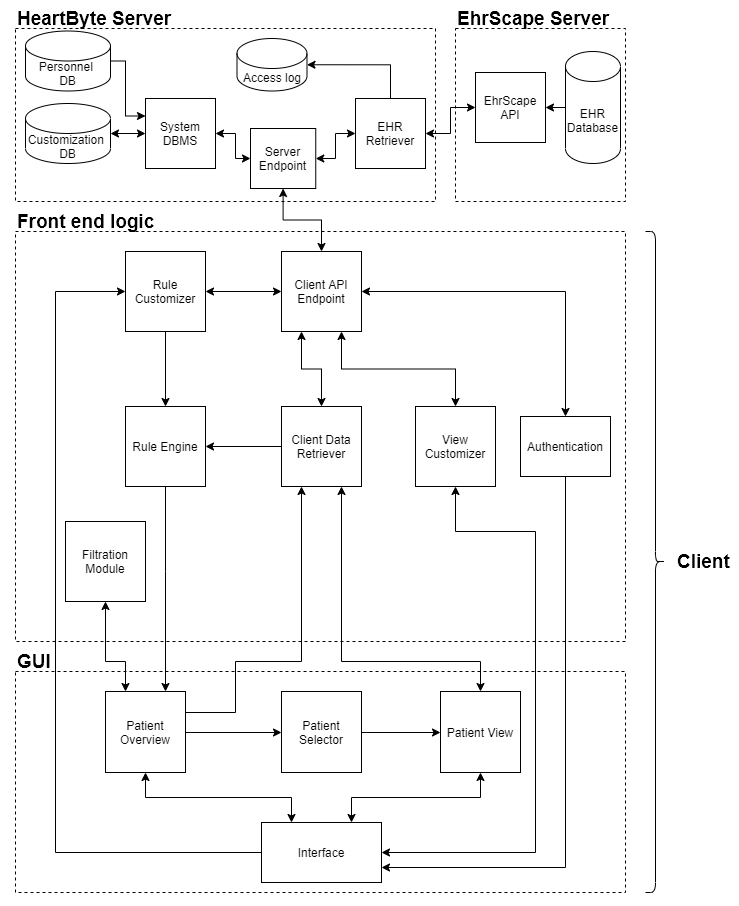
\includegraphics[width=15cm]{architecture.png}
    \caption{Box and line diagram illustrating layers of the system and its submodules}
    \label{fig: boxAndLineDiag}
\end{figure}

\section{Product functions} 
HeartByte’s web application provides an overview of patients self-monitoring their health in which the user of the application will be able to clearly see and efficiently manage all patients in their healthcare center or subunit within RÖ. Patients can be sorted and filtered by different criteria, which will aid the user in the navigation between patients. Health prioritization levels set by a specific healthcare center or subunit will effectively present the patients in most need of care for the health care staff, as well as alert the staff when appropriate actions need to be taken. Admins can set at which values the system will trigger a change in the patient’s priority level. Views in the application can be customized based on for instance diagnosis and team. When a specific patient is accessed the user is presented with detailed information about the patient in question. Detailed information includes measured health data, current medication, contact information, medical information, activity history, scheduled appointments and so on. Furthermore, for each patient the measured health data is presented with interactive graphs of the measured health data to aid the health care staff in their assessment and understanding of a patient’s health situation. 
\newline
\newline
Some significant functions included in HeartByte’s system are illustrated in Figure \ref{fig: useCaseDiag}. The use case diagram is not a complete representation of all functions provided by HeartByte’s system but it rather represents a general overview of significant functions. The use case diagram is further described in the Architecture Notebook \cite{architecture}.

Listed below as user stories are the significant functions of HeartByte’s web application:
\newline
\newline
\textbf{U1:} As a health care worker, I want to see an clear overview of many patients so that I can manage many patients under care.
\newline
\newline
\textbf{U2:} As a health care worker, I want to be able to sort patients by ‘Namn’, ‘Personnummer’, ‘Prioritet’, ‘Diagnos’ and ‘Senast Uppdaterad’ so that I can efficiently navigate through many patients.
\newline
\newline
\textbf{U3:} As a health care worker, I want to be able to filter patients by ‘Ålder’, ‘Prioritering’, ‘Verksamhet’, ‘Team’, ‘Avdelning’ and ‘Diagnos’ so that I can quickly find patients.
\newline
\newline
\textbf{U4:} As a health care worker, I want to prioritize patients so that patients in most need of care receive medical attention first.
\newline
\newline
\textbf{U5:} As a health care giver, I want to see detailed information about a patient so that I can provide proper care.
\newline
\newline
\textbf{U6:} As health care giver, I want to see a patient’s measured health data so that I can correctly assess the health of patients.
\newline
\newline
\textbf{U7:} As a health care giver, I want to see a patient’s diagnoses and medications so that I can adequately treat patients. 
\newline
\newline
\textbf{U8:} As a health care giver, I want to see a patient's contact information so that I can contact patients.
\newline
\newline
\textbf{U9:} As health care worker or admin, I want to be able to log in and log out of the system so that I can securely use the system.
\newline
\newline
\textbf{U10:} As an admin, I want to customize prioritization rules for patients so that health care workers can treat patients according to the level of health urgency. 
\newline
\newline
\textbf{U11:} As an admin, I want to customize views so that health care workers can effectively manage many patients. 
\begin{figure}[htp]
    \centering
    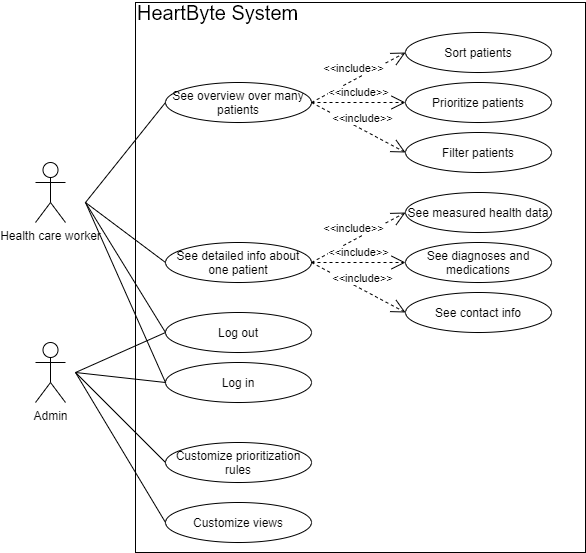
\includegraphics[width=15cm]{useCase.png}
    \caption{Use case diagram of significant functions}
    \label{fig: useCaseDiag}
\end{figure}

\section{User Characteristics}
The users of HeartByte’s system are either administrators or users, as defined in section~\ref{section:def}. Administrators are users with extended system capabilities. Administrators can set health prioritization rules for patients and customize views according to the guidelines set by a health care center or subunit within RÖ. All users of HeartByte’s system are expected to have a certain level of medical competence to use the system as intended, that is to provide safe and proper care for patients enrolled in RÖ’s self-monitoring program.


\section{Constraints}
The main constraint for this product concerns confidentiality and security. Since this product is designed to be used by health care providers there are some regulations concerning patient data security, such as "patientdatalagen". These regulations mainly affect patient data confidentiality and what health care staff should have access to what patient information.

\section{Assumptions and dependencies}
An assumption is that the system will be used on computers and tablets with a web browser. Since HeartByte's system requires the user to be logged in in the system to access any functionality it is also assumed that the user has logged in.

The system needs to interact with other systems to function. OAuth is to be used for authentication and log in functionality. The system will also need to interact with an OpenEHR-database to access and store EHRs. 

%"This subsection of the SRS should list each of the factors that affect the requirements stated in the SRS. These factors are not design constraints on the software but are, rather, any changes to them that can affect the requirements in the SRS. For example, an assumption may be that a specific operating system will be available on the hardware designated for the software product. If, in fact, the operating system is not available, the SRS would then have to change accordingly."

%\section{Apporting of requirements}
%There are some requirements that could be delayed until future versions of the systems if the project is delayed.

\chapter{Specific requirements}
This chapter contains the software requirements and gives a detailed
description of the system and its features. 

\section{Interface requirements}
The main system interface is the user interface. The user interfaces are divided into two subsections: the user view and the admin view. The admin has, as previously mentioned, every functionality the user has. Meanwhile the user lacks som functionality that only an admin has access to. 

\subsection{User interfaces -  User View}
This section describes the user interfaces as the pages/views defined in the "Hi-Fi 2.1" document \cite{prototype}.

\subsubsection{Login page}
\begin{figure}[h!]
    \centering
    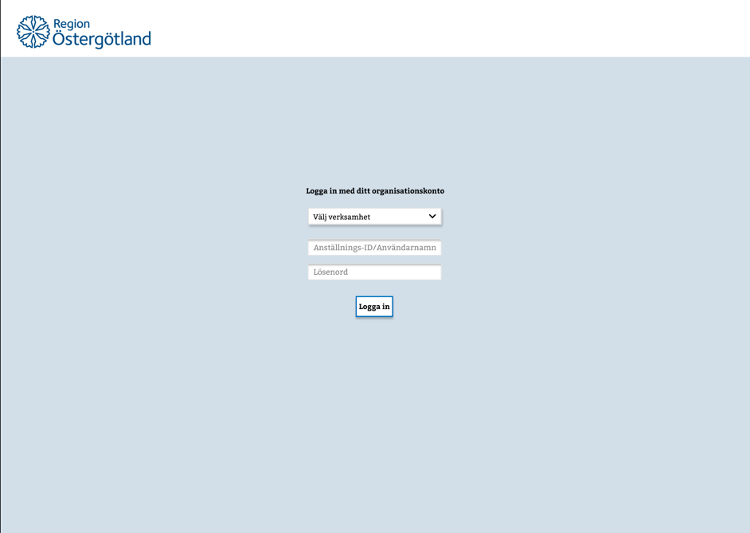
\includegraphics[width=15cm]{login.png}
    \caption{Login page}
    \label{fig: login}
\end{figure}

First page shown when signing in to the system. Start by selecting the operation and then log in with the employment-ID or username and then enter a password. See Figure \ref{fig: login}. Successful login with OAuth leads to the “Mina Patienter” page. 

\subsubsection{Patient view}
The individual patient view is divided into several tabs: "Mätvärden", "Översikt", "Läkmedelslista" and  "Kalender". The following sections are based on these tabs. 

\subsubsection{"Mätvärden"}
\begin{figure}[h!]
    \centering
    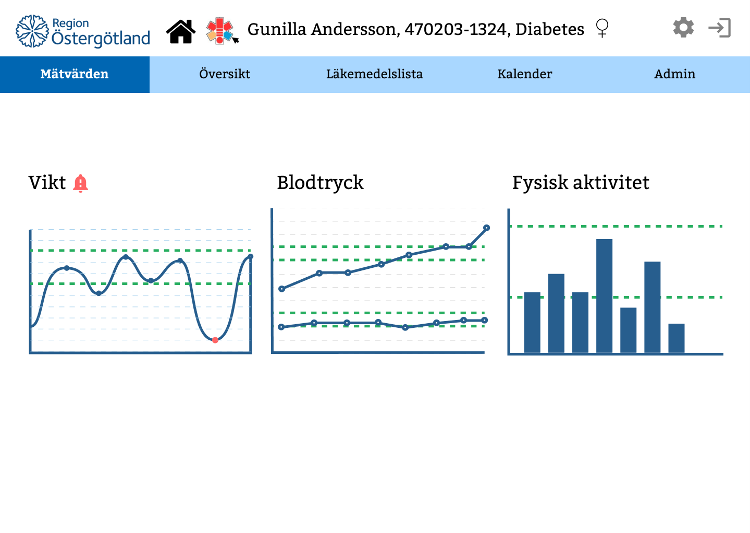
\includegraphics[width=15cm]{meas.png}
    \caption{Measurements}
    \label{fig: meas}
\end{figure}

\begin{figure}[h!]
    \centering
    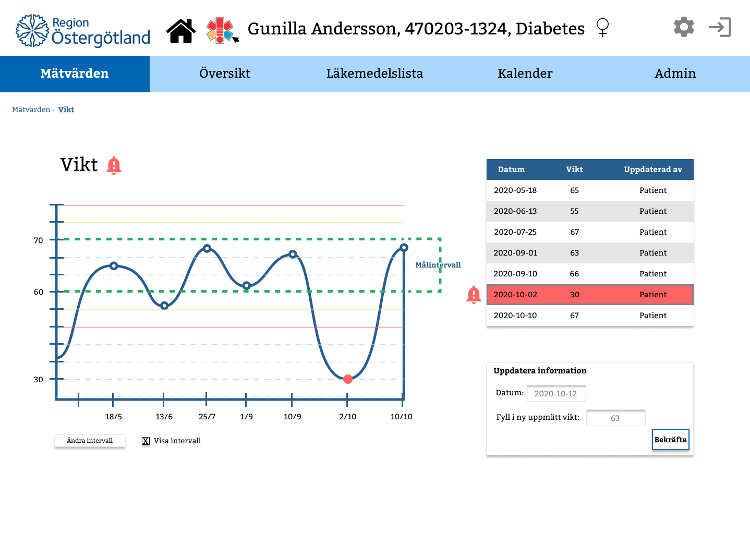
\includegraphics[width=15cm]{measweight.png}
    \caption{Measurements Weight}
    \label{fig: measweight}
\end{figure}
All the current measurements for the specific patient are displayed in graphs. Warning symbols if something needs to be handled. See Figure \ref{fig: meas}.
The graphs in the first page of the measurement are displayed with only a target range. When entering a specific measurement, see Figure \ref{fig: measweight}, intervals are also shown for what triggers yellow and red notifications. This is shown by default, but the user can choose to not display the intervals by clicking the check box “Visa intervall”. The "Ändra intervall"-button in Figure \ref{fig: measweight} is not visible for regular users.

\clearpage

\subsubsection{"Översikt"}
\begin{figure}[h!]
    \centering
    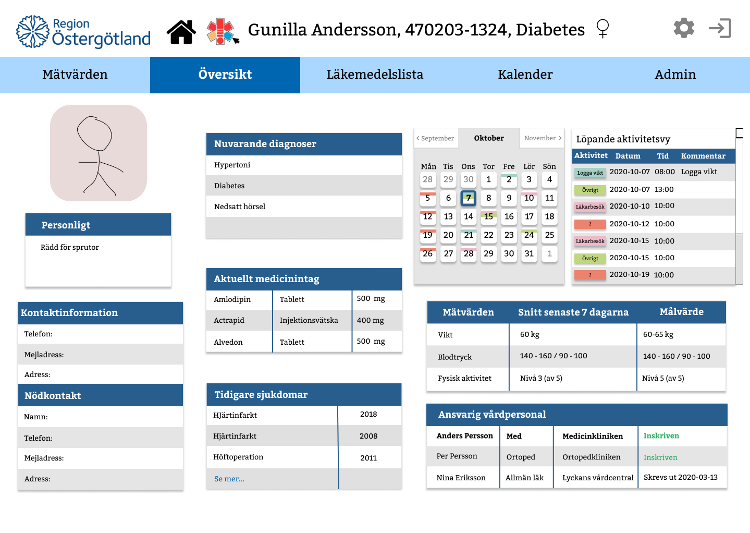
\includegraphics[width=15cm]{patoverview.png}
    \caption{Patient overview}
    \label{fig: patoverview}
\end{figure}
Information about the specific patient with contact information and emergency contact. Shows current diagnoses, current medication intake, average of current measurement values, previous diagnoses and caregivers and staff who handle the patient. Picture of the specific patient.

The tables length is adapted to the number of diagnoses, medications, measurements, responsible staff members etc. 

Table of “tidigare sjukdomar” is shown with a maximum of 4 rows with the see more text included. When pressing see more, the table expands in length and shows the rest of the information.


\clearpage

\subsubsection{"Läkemedelslista"}
\begin{figure}[h!]
    \centering
    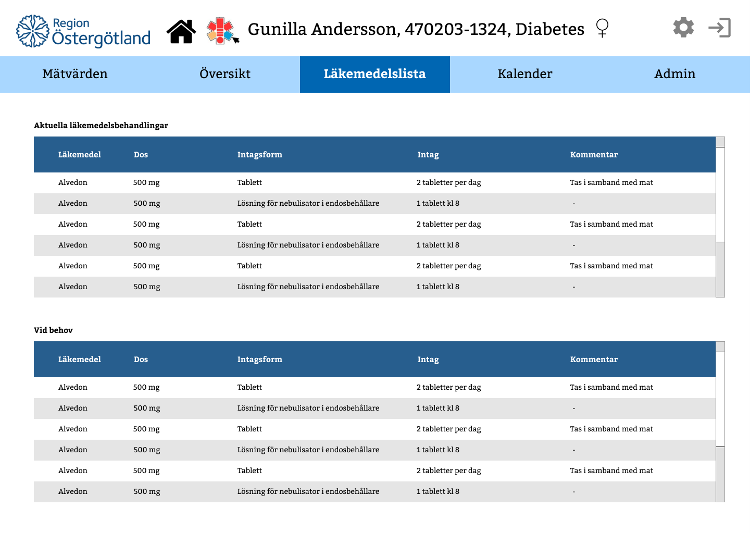
\includegraphics[width=15cm]{medications.png}
    \caption{Medications list}
    \label{fig: medications}
\end{figure}
Table of medicines that shows current/relevant medication intake for a specific patient and a table of medicines that a specific patient can take if necessary.

\clearpage

\subsubsection{"Kalender"}
\begin{figure}[h!]
    \centering
    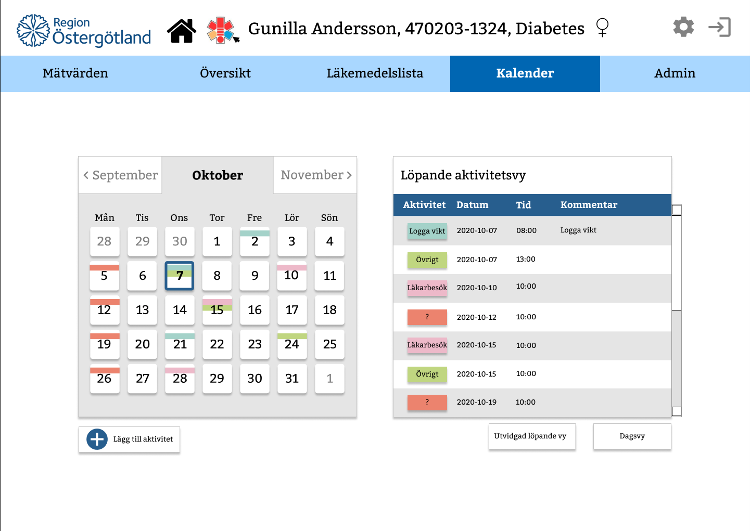
\includegraphics[width=15cm]{patcalendar.png}
    \caption{Patient Calendar}
    \label{fig: patcalendar}
\end{figure}

Displays a calendar view over a month. When interacting with a specific day in the calendar the booked activities are displayed in a view in a table next to it. All the upcoming activities are also shown in the table that you can scroll. By default, the current day is displayed. Ability to choose a day view or a view with a list of all the upcoming activities (this should be the default view). The tables are possible to expand. Ability to add activities into the calendar, this function is not necessary to build, can only show the button.


\subsubsection{Overview}
The overview of patients is also divided into several tabs: "Mina Patienter", "Alla Patienter", "Notislogg" and "Kalender". The following sections are based on these tabs. 

\subsubsection{"Mina Patienter"}
\begin{figure}[h!]
    \centering
    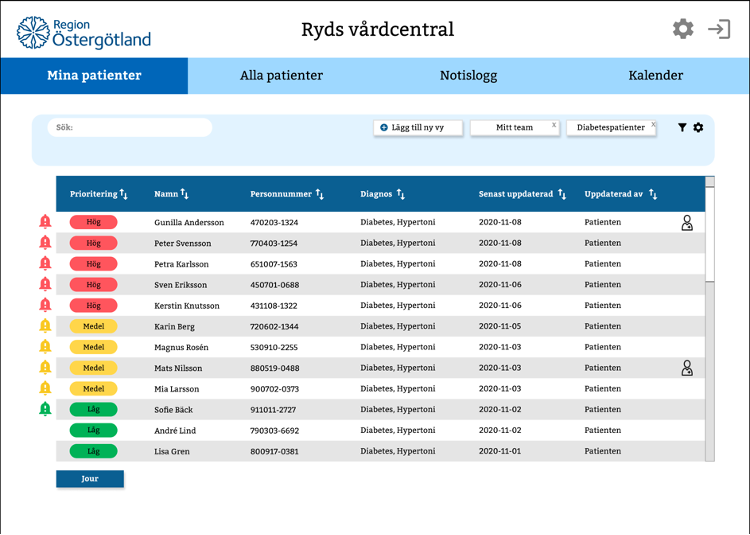
\includegraphics[width=15cm]{mypat.png}
    \caption{My Patients}
    \label{fig: mypat}
\end{figure}

\begin{figure}[h!]
    \centering
    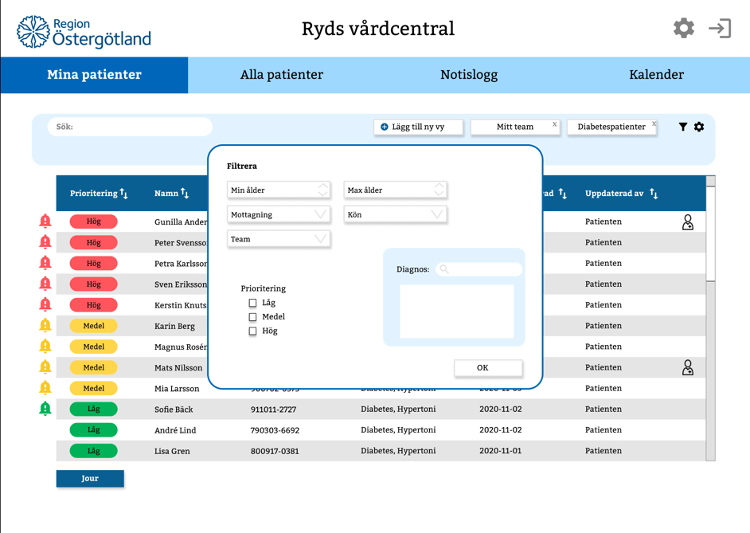
\includegraphics[width=15cm]{mypatfilter.png}
    \caption{My Patients Filter}
    \label{fig: mypatfilter}
\end{figure}

\begin{figure}[h!]
    \centering
    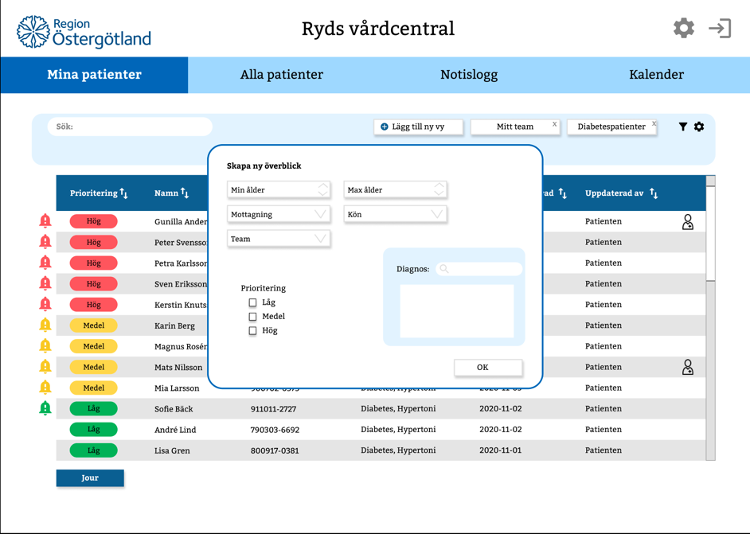
\includegraphics[width=15cm]{createnewview.png}
    \caption{Create new view}
    \label{fig: createnewview}
\end{figure}

Shows table of all patients in the system connected to the department you are logged in to. See Figure \ref{fig: mypat}. Ability to search for specific patients and filter and sort the list. See Figure \ref{fig: mypatfilter} for filter function. The sort functions are placed on each heading in the table. Doctors icons in the table show who is handling the notification.

Ability to add new views visible only to the currently logged in user, can add up to 7 views, so there will be 4 buttons on top (including the “lägg till ny vy” button) and 4 buttons under when adding more. Also ability to remove these filters by clicking on “X”. See Figure \ref{fig: createnewview}

The gear icon in the filter/search box is not visible for users.


\clearpage

\subsubsection{"Alla Patienter"}
\begin{figure}[h!]
    \centering
    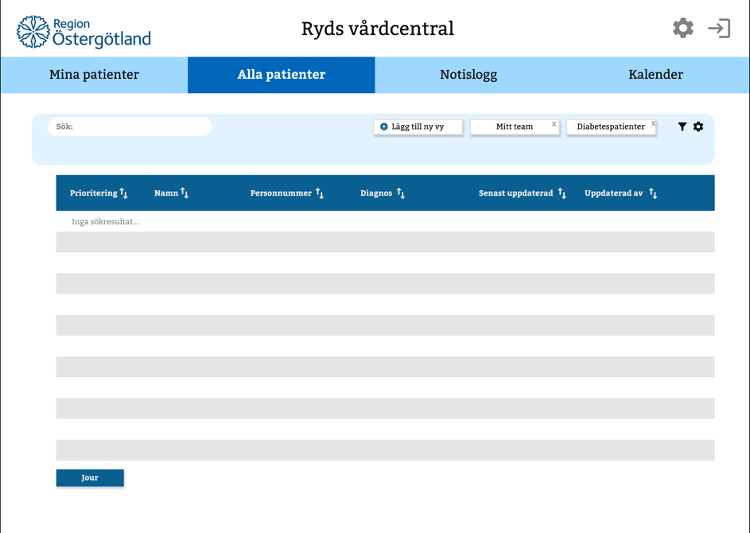
\includegraphics[width=15cm]{allpat.png}
    \caption{All Patients}
    \label{fig: allpat}
\end{figure}

\begin{figure}[h!]
    \centering
    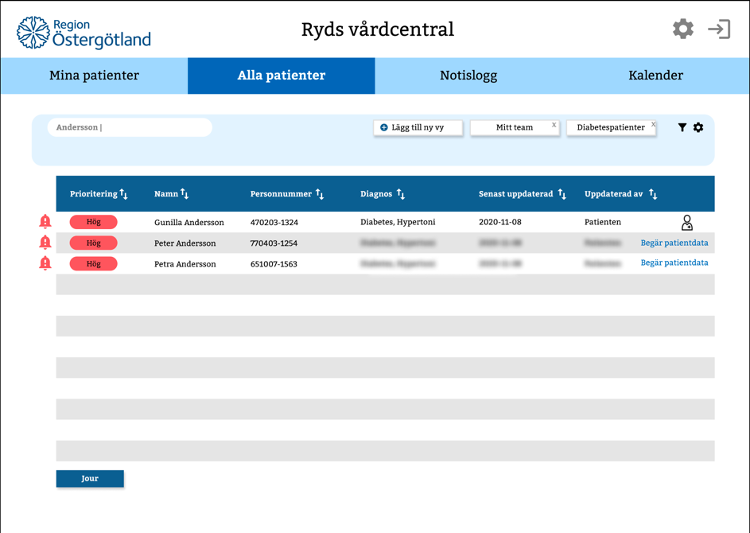
\includegraphics[width=15cm]{allpatdiabetes.png}
    \caption{All Patients Specific View}
    \label{fig: allpatdiabetes}
\end{figure}
Can show all the patients in the system. Patients are shown in the table when searched for. The information of patients the user does not have access to that can be shown is the name, social security number and level of alertness. The rest of the information of the patients to whom the user does not have access shall be blurred, until the user has asked for permission to access said information. 

\clearpage

\subsubsection{"Notislogg"}
\begin{figure}[h!]
    \centering
    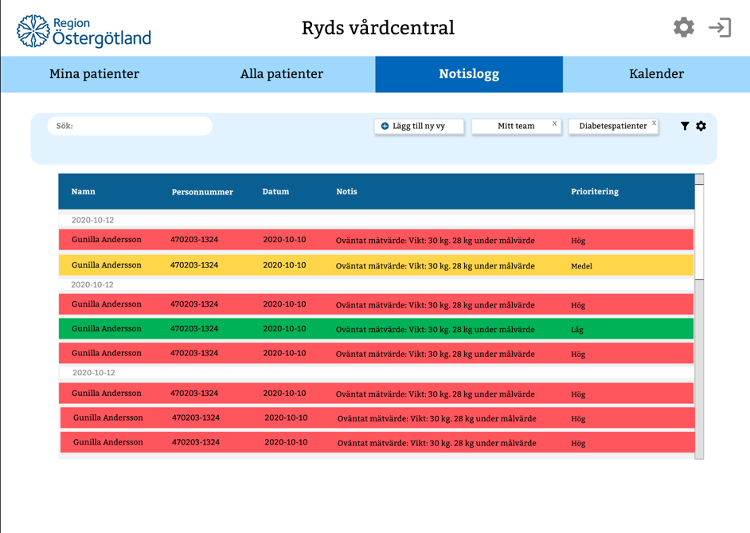
\includegraphics[width=15cm]{notifications.png}
    \caption{Notifications}
    \label{fig: notifications}
\end{figure}
All the activities that happen are gathered in this notification log with a prioritization of how important the notification is to be handled. For example, if a measured value is taken with a large deviation from the average value, this should indicate a high prioritized notification.
Same sorting and search box as in “Mina patienter” and “Alla patienter”.


\subsubsection{"Kalender"}
The difference between this calendar and the calendar under the patient specific view, see Figure \ref{fig: patcalendar}, is that the calendar for the logged-in staff is displayed here. Therefore, the activities displayed in the patient specific calendar will differ from those activities that will appear in this calendar. Here activities will be about booked meetings with patients. 

\subsection{User interfaces -  Admin View}
\label{section: admin}
This section describes the admin views as defined in the "Hi-Fi" document \cite{prototype}. As the admin has the same functionality as the user only the functionality the user does not have access to but the admin does is described in this section. The section is divided into different subsections based on the system's different pages.

\subsubsection{"Översikt"}
\begin{figure}[h!]
    \centering
    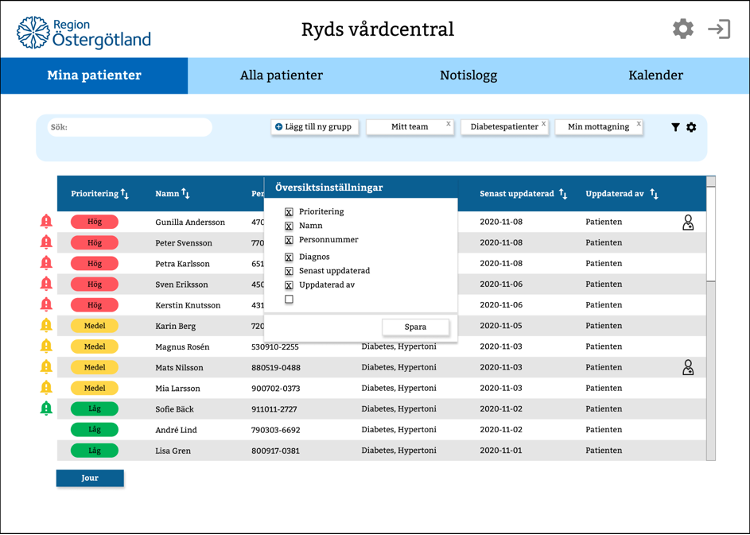
\includegraphics[width=15cm]{mypatsettings.png}
    \caption{My Patients Settings}
    \label{fig: mypatsettings}
\end{figure}

The gear icon in the filter/search box is only visible for admins and leads to a pop-up window of display settings "Översiktsinställningar" where the admin can determine which columns shall be visible in the dashboard, see Figure \ref{fig: mypatsettings}.

\subsubsection{"Patient"}
\begin{figure}[h!]
    \centering
    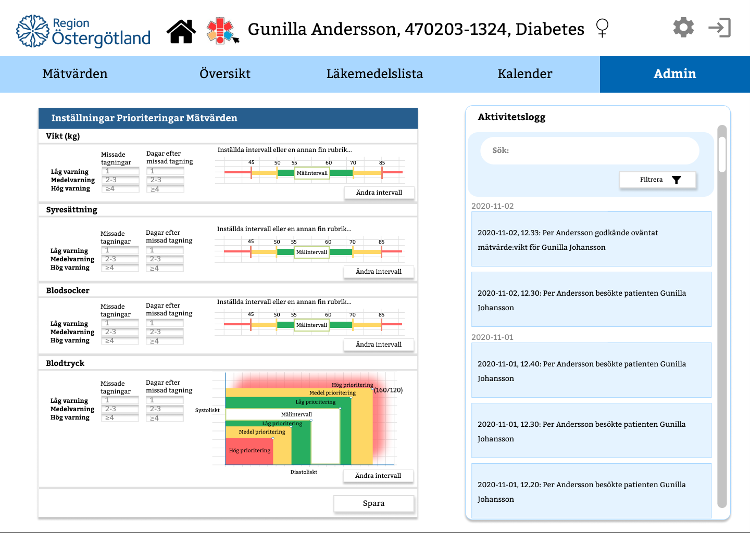
\includegraphics[width=15cm]{patadmin.png}
    \caption{Patient - Admin}
    \label{fig: patadmin}
\end{figure}

Page only visible for admins. See Figure \ref{fig: patadmin}.

"Inställningar Prioriteringar Mätvärden"
Set the settings for intervals on the patient measurements. For changing the intervals you press “Ändra intervall” and are directed to the measurement page where you can change the interval and seeing the graph and measurements at the same time. The the user presses “Ändra intervall” once on admin page to see the setting in measurement.

"Aktivitetslogg"
Shows all the activity that happens on a patient specific page. All activities must be logged for the patient's integrity. The admin shall be able to sort and filter activity log in order to find specific logs.

\subsubsection{"Mätvärden"}
In the page "Mätvärden" only admins have a visible  “Ändra intervall”-button. When interacting with the button, the interval setting is displayed next to the graph. See Figure \ref{fig: measweight}.


%\subsection{Software interfaces}
%Same as 2.1???? 

%\subsection{Hardware interfaces}
%\subsection{Communication interfaces}


\section{Functional requirements}
The following section includes the requirements that specify all the fundamental actions of the software system. The section is divided into four main categories: "Admin", "Patient", "System" and "Översikt". These categories are then divided into subcategories based on the different views in each category. 
\\ \\
To clarify how the requirements presented in tables see explanation below. 

\begin{center}
\begin{tabularx}{\linewidth}{| s | m | m | b | s |}
\hline
\textbf{ID:} & \textbf{Title} & \textbf{Precondition} & \textbf{Description} & \textbf{Priority} \\
\hline
FRXXX id of requirement & 
Title to briefly explain the requirement & 
Explains any preconditions for requirement & 
Description of what will happen in the system.  
    \newline \textbf{Input:} What triggers the function  
    \newline \textbf{Action:} How the system responds to the input 
    \newline \textbf{Output:} The function's output &
Priority level (Low-Medium-High) \\ 
\hline
\end{tabularx}
\end{center}

\subsection{Admin}
In section 3.2.1. we describe functional requirements for the Admin. A precondition is that the admin is logged in to the system. 

\subsubsection{Översikt/Notislogg}
A precondition is that the admin is logged in and on the view “Oversikt/Notislogg”
\begin{center}
\begin{tabularx}{\linewidth}{| s | m | m | b | s |}
\hline
\textbf{ID:} & \textbf{Title} & \textbf{Precondition} & \textbf{Description} & \textbf{Priority} \\
\hline
FR001 & 
Create new view & 
& 
\textbf{Input:} Button with ID = "adminOverviewNotisNewViewBtn" is pressed 
    \newline \textbf{Action:} System loading new window with customization settings
    \newline \textbf{Output:} Pop-up window with ID = "adminOverviewNotisNewViewPopupWindow" is displayed &
Medium \\ 
\hline
FR002 & 
Customization of overview dashboard &
FR089 is fulfilled & 
\textbf{Input:} Choose between different checkboxes of display columns with ID:(Namn, Personnummer, Priority, Diagnos, Senast Uppdaterad, Uppdaterad av, Team). Click on save-button with ID = "adminFilterSave".
    \newline \textbf{Action:} The system generates and saves display-settings.
    \newline \textbf{Output:} Overview dashboard updated according to selected settings.
    & 
Medium \\
\hline
FR046 & 
Create new customized view based on age & 
FR001 is fulfilled &  
    \newline \textbf{Input:} Minimum age and maximum age in text fields with ID = "minage" \& "maxage" and presses button "OK" with ID = "okView". 
    \newline \textbf{Action:} System generates new view based on age settings and saves to database.
    \newline \textbf{Output:} System displays a pop-up window with ID = "adminOverviewNotisConfirmView"
    & 
Medium \\
\hline
FR047 & 
Create new customized view based on gender & 
FR001 is fulfilled &  
    \newline \textbf{Input:} Click on dropdown menu "Kön" with ID = "gender" and choose between "Alla" (ID = "all"), "Man" (ID = "male") or "Kvinna" (ID = "female") and presses button "OK" with ID = "okView".
    \newline \textbf{Action:}  System generates new view based on gender settings and saves to database.
    \newline \textbf{Output:} System displays a pop-up window with ID = "adminOverviewNotisConfirmView"
    & 
Medium \\
\hline
FR048 & 
Create new customized view based on team & 
FR001 is fulfilled &  
    \newline \textbf{Input:} Click on dropdown menu "Team" with ID = "teammenu" and choose between "Alla" (ID = "all"),  or "Team$<x>$" (ID = "team$<x>$"), where x is a unique integer, and presses button "OK" with ID = "okView".
    \newline \textbf{Action:} System generates new view based on team settings and saves to database.
    \newline \textbf{Output:} System displays a pop-up window with ID = "adminOverviewNotisConfirmView"
    & 
Medium \\
\hline
FR049 & 
Create new customized view based on department & 
FR001 is fulfilled &  
    \newline \textbf{Input:} Click on dropdownmenu with ID = "departmentMenu" and choose between "Alla" (ID = 'all'), Department 1 (ID = 'Department1) or Department 2 (ID = 'Department2') and presses button "OK" with ID = "okView".
    \newline \textbf{Action:} System generates new view based on age settings and saves to database.
    \newline \textbf{Output:} System displays a pop-up window with ID = "adminOverviewNotisConfirmView"
    & 
Medium \\
\hline
FR050 & 
Create new customized view based on priority  & 
FR001 is fulfilled &  
    \newline \textbf{Input:} Priority level selected in checkboxes (Low, Medium, High) and presses button "OK" with ID = "okView". 
    \newline \textbf{Action:} System generates new view based on priority settings and saves to database.
    \newline \textbf{Output:} System displays a pop-up window with ID = "adminOverviewNotisConfirmView" 
    & 
Medium \\
\hline
FR051 & 
Create new customized view based on diagnosis  & 
FR001 is fulfilled &  
    \newline \textbf{Input:} Diagnosis in text field with ID "customizeViewDiagnosis" OR click on the diagnosis  checkbox with ID = $<diagnosis>$ and press button "OK" with ID = "okView".
    \newline \textbf{Action:} System generates new view based on diagnosis settings and saves to database.
    \newline \textbf{Output:} System displays a pop-up window with ID = "adminOverviewNotisConfirmView"
    & 
Medium \\
\hline
FR052 & 
Confirm created view & 
FR001, FR046-Fr051 are fulfilled &  
    \newline \textbf{Input:} Title of new view in text field with ID "saveNewView", the selected user group in drop-down menu with ID "viewAvailableFor" and sign button with ID "confirmCustomizedView"
    \newline \textbf{Action:}  System generates new view based on previously selected settings and saves to database.
    \newline \textbf{Output:} New view available for all users in the chosen user group.
    & 
Medium \\
\hline
FR089 & 
Overview dashboard settings & 
&  
\textbf{Input}: Click on the settings button with ID ="adminOverviewNotisCustomizeSettingsDashboardBtn"
\newline \textbf{Action}: System generates popup window
\newline \textbf{Output}: System displays customization popup window with ID = "adminOverviewNotisCustomizeSettingsPopupWindow"
    & 
Medium \\
\hline
\end{tabularx}
\end{center}

\subsubsection{Översikt/Mina-Patienter}
A precondition is that the admin is logged in and on the view “Översikt/Mina-Patienter”
\begin{center}
\begin{tabularx}{\linewidth}{| s | m | m | b | s |}
\hline
\textbf{ID:} & \textbf{Title} & \textbf{Precondition} & \textbf{Description} & \textbf{Priority} \\
\hline
FR003 & 
Create new view &
& 
\textbf{Input:} Button with ID = "adminOverviewMyPatientsNewViewBtn" is pressed
    \newline \textbf{Action:} System loading new window with customization settings
    \newline \textbf{Output:} Pop-up window with ID "adminOverviewMyPatientsNewViewPopupWindow" is displayed &
Medium \\ 
\hline
FR004 & 
Customization of overview dashboard &
FR090 is fulfilled & 
\textbf{Input:} Choose between different checkboxes of display columns (Namn, Personnummer, Priority, Diagnos, Senast Uppdaterad, Uppdaterad av, Team). Click on save-button with ID = "adminFilterSave".
    \newline \textbf{Action:} System displays customization popup window. The system generates and saves display-settings
    \newline \textbf{Output:} Overview dashboard updated according to selected settings. & 
Medium \\
\hline
FR038 & 
Create new customized view based on age & 
FR003 is fulfilled &  
    \textbf{Input:} Minimum age and maximum age in text fields with ID = "minage" \& "maxage" and presses button "OK" with ID = "okView". 
    \newline \textbf{Action:} System generates new view based on age settings and saves to database.
    \newline \textbf{Output:} System displays a pop-up window with ID = "adminOverviewMyPatientsConfirmView" 
    & 
Medium \\
\hline
FR039 & 
Create new customized view based on gender & 
FR003 is fulfilled &  
    \textbf{Input:} Click on dropdown menu "Kön" with ID = "gender" and choose between "Alla" (ID = "all"), "Man" (ID = "male") or "Kvinna" (ID = "female") and presses button "OK" with ID = "okView".
    \newline \textbf{Action:}  System generates new view based on gender settings and saves to database.
    \newline \textbf{Output:} System displays a pop-up window with ID = "adminOverviewMyPatientsConfirmView" 
    & 
Medium \\
\hline
FR040 & 
Create new customized view based on team & 
FR003 is fulfilled &  
    \textbf{Input:} Click on dropdown menu "Team" with ID = "teammenu" and choose between "Alla" (ID = "all"),  or "Team$<x>$" (ID = "team$<x>$"), where x is a unique integer, and presses button "OK" with ID = "okView".
    \newline \textbf{Action:} System generates new view based on team settings and saves to database.
    \newline \textbf{Output:} System displays a pop-up window with ID = "adminOverviewMyPatientsConfirmView" 
    & 
Medium \\
\hline
FR041 & 
Create new customized view based on department & 
FR003 is fulfilled &  
    \textbf{Input:} Click on dropdownmenu with ID = "departmentMenu" and choose between "Alla" (ID = 'all'), Department 1 (ID = 'Department1) or Department 2 (ID = 'Department2') and presses button "OK" with ID = "okView".
    \newline \textbf{Action:} System generates new view based on age settings and saves to database.
    \newline \textbf{Output:} System displays a pop-up window where the user must confirm the new view. 
    & 
Medium \\
\hline
FR042 & 
Create new customized view based on priority  & 
FR003 is fulfilled &  
    \textbf{Input:} Priority level selected in checkboxes (Low, Medium, High) and presses button "OK" with ID = "okView". 
    \newline \textbf{Action:} System generates new view based on priority settings and saves to database.
    \newline \textbf{Output:} System displays a pop-up window with ID = "adminOverviewMyPatientsConfirmView" 
    & 
Medium \\
\hline
FR043 & 
Create new customized view based on diagnosis  & 
FR003 is fulfilled &  
    \textbf{Input:} Diagnosis in text field with ID "customizeViewDiagnosis" OR click on the diagnosis  checkbox with ID = $<diagnosis>$ and press button "OK" with ID = "okView".
    \newline \textbf{Action:} System generates new view based on diagnosis settings and saves to database.
    \newline \textbf{Output:} System displays a pop-up window with ID = "adminOverviewMyPatientsConfirmView"
    & 
Medium \\
\hline
FR044 & 
Confirm created view & 
FR003, FR038-FR043 are fulfilled. In view with ID = "adminOverviewMyPatientsConfirmView". &  
    \textbf{Input:} Title of new view in text field with ID "saveNewView", the selected user group in drop-down menu with ID "viewAvailableFor" and sign button with ID "confirmCustomizedView"
    \newline \textbf{Action:}  System generates new view based on previously selected settings and saves to database.
    \newline \textbf{Output:} New view available.
    & 
Medium \\
\hline
Fr090 & 
Overview dashboard settings & 
& 
\textbf{Input}: Click on the settings button with ID ="adminOverviewMyPatientsCustomizeSettingsDashboardBtn"
\newline \textbf{Action}: System generates popup window
\newline \textbf{Output}: System displays customization popup window with ID = "adminOverviewMyPatientsCustomizeSettingsPopupWindow" & 
Medium \\
\hline
\end{tabularx}
\end{center}

\subsubsection{Översikt/Alla-Patienter}
A precondition is that the admin is logged in and on the view “Översikt/Alla-Patienter”

\begin{center}
\begin{tabularx}{\linewidth}{| s | m | m | b | s |}
\hline
\textbf{ID:} & \textbf{Title} & \textbf{Precondition} & \textbf{Description} & \textbf{Priority} \\
\hline
FR053 & 
Create new view &
 & 
\textbf{Input:} Button with ID = "adminOverviewAllPatientsNewViewBtn is pressed 
    \newline \textbf{Action:} System loading new window with customization settings
    \newline \textbf{Output:} Pop-up window with ID "adminOverviewAllPatientsNewViewPopupWindow" is displayed &
Medium \\ 
\hline
FR054 & 
Create new customized view based on age & 
FR053 is fulfilled &  
    \textbf{Input:} Minimum age and maximum age in text fields with ID = "minage" \& "maxage" and presses button "OK" with ID = "okView".
    \newline \textbf{Action:} System generates new view based on age settings and saves to database.
    \newline \textbf{Output:} System displays a pop-up window with ID = "adminOverviewAllPatientsConfirmView" 
    & 
Medium \\
\hline
FR055 & 
Create new customized view based on gender & 
FR053 is fulfilled &  
    \textbf{Input:} Click on dropdown menu "Kön" with ID = "gender" and choose between "Alla" (ID = "all"), "Man" (ID = "male") or "Kvinna" (ID = "female") and presses button "OK" with ID = "okView".
    \newline \textbf{Action:}  System generates new view based on gender settings and saves to database.
    \newline \textbf{Output:}  System displays a pop-up window with ID = "adminOverviewAllPatientsConfirmView"
    & 
Medium \\
\hline
FR056 & 
Create new customized view based on team & 
FR053 is fulfilled &  
    \textbf{Input:} Click on dropdown menu "Team" with ID = "teammenu" and choose between "Alla" (ID = "all"),  or "Team$<x>$" (ID = "team$<x>$"), where x is a unique integer, and presses button "OK" with ID = "okView".
    \newline \textbf{Action:} System generates new view based on team settings and saves to database.
    \newline \textbf{Output:} System displays a pop-up window with ID = "adminOverviewAllPatientsConfirmView"
    & 
Medium \\
\hline
FR057 & 
Create new customized view based on department & 
FR053 is fulfilled &  
    \textbf{Input:} Click on dropdownmenu with ID = "departmentMenu" and choose between "Alla" (ID = 'all'), Department 1 (ID = 'Department1) or Department 2 (ID = 'Department2') and presses button "OK" with ID = "okView".
    \newline \textbf{Action:} System generates new view based on age settings and saves to database.
    \newline \textbf{Output:} System displays a pop-up window with ID = "adminOverviewAllPatientsConfirmView" 
    & 
Medium \\
\hline
FR058 & 
Create new customized view based on priority  & 
FR053 is fulfilled &  
    \textbf{Input:} Priority level selected in checkboxes (Low, Medium, High) and presses button "OK" with ID = "okView". 
    \newline \textbf{Action:} System generates new view based on priority settings and saves to database.
    \newline \textbf{Output:} System displays a pop-up window with ID = "adminOverviewAllPatientsConfirmView"
    & 
Medium \\
\hline
FR059 & 
Create new customized view based on diagnosis  & 
FR053 is fulfilled &  
    \textbf{Input:} Diagnosis in text field with ID "customizeViewDiagnosis" OR click on the diagnosis  checkbox with ID = $<diagnosis>$ and press button "OK" with ID = "okView".
    \newline \textbf{Action:} System generates new view based on diagnosis settings and saves to database.
    \newline \textbf{Output:} System displays a pop-up window with ID = "adminOverviewAllPatientsConfirmView"
    & 
Medium \\
\hline
FR060 & 
Confirm created view & 
FR053-Fr059, FR092 are fulfilled &  
    \textbf{Input:} Title of new view in text field with ID "AdminAllpatientsSaveNewView", the selected user group in drop-down menu with ID "viewAvailableFor" and sign button with ID "confirmCustomizedView"
    \newline \textbf{Action:}  System generates new view based on previously selected settings and saves to database.
    \newline \textbf{Output:} New view available for all users in the chosen user group.
    & 
Medium \\
\hline
FR061 & 
Customization of overview dashboard &
FR091 is fulfilled & 
\textbf{Input:} Choose between different checkboxes of display columns (Namn, Personnummer, Priority, Diagnos, Senast Uppdaterad, Uppdaterad av, Team). Click on save-button with ID = "adminFilterSave".
    \newline \textbf{Action:} The system generates and saves display-settings
    \newline \textbf{Output:} Overview dashboard updated according to selected settings. & 
Medium \\
\hline
FR91 & 
Overview dashboard settings &
 & 
\textbf{Input:}  Click on the settings button with ID ="adminOverviewAllPatientsCustomizeSettingsDashboardBtn"
\newline \textbf{Action:} System generates popup window
\newline \textbf{Output:} System displays customization popup window with ID = "adminOverviewAllPatientsCustomizeSettingsPopupWindow"& 
Medium \\
\hline
FR92 & 
Create new customized view based on operation &
FR053 is fulfilled & 
\textbf{Input:} Click on dropdownmenu with ID = "operationMenu" and choose between "Alla" (ID = 'all'), Operation 1 (ID = 'Operation1) or Operation 2 (ID = 'Operation2') and presses button "OK" with ID = "okView".
\newline \textbf{Action:} System generates new view based on operation settings and saves to database.
\newline \textbf{Output:} System displays a pop-up window with ID = "adminAllPatientsViewConfirm" & 
Medium \\
\hline
\end{tabularx}
\end{center}

\subsubsection{Patient/Admin}
A precondition is that the admin is logged in and on the view “Patient/Admin” 

\begin{center}
\begin{tabularx}{\linewidth}{| s | m | m | b | s |}
\hline
\textbf{ID:} & \textbf{Title} & \textbf{Precondition} & \textbf{Description} & \textbf{Priority} \\
\hline
FR006 & 
Configure values for the rule engines priority & 
 & 
    \textbf{Input}: Enter limit values for different measurements in text fields with specific IDs and click "save"-button with ID = "patientViewAdminBtnValue".
    \newline \textbf{Action}: System saves and sets patient specific prioritization limits.
    \newline \textbf{Output}: Settings displayed &
High \\ 
\hline 
FR007 & 
Accessing activity log & 
 & 
\textbf{Input}: Click on ""Admin"" tab with ID: = "patientViewAdminTabBtn" \newline
\textbf{Action}: Load activity log from database \newline 
\textbf{Output}: Display activity log &
Medium \\ 
\hline 
FR008 & 
Search in activity log & 
 & 
\textbf{Input}: Text string (search parameter) in search box with ID = "patientViewAdminActivityField" \newline 
\textbf{Action}: System checks for activities or users that matches text string \newline 
\textbf{Output}: Displays activities and/or users that matches string. &
Low \\ 
\hline
FR009 & 
Filter in activity log & 
Filter-button with ID ="patientAdminFilterBtn" has been pressed and system currently displays "Filter" window (ID = "patientAdminFilterWindow").  & 
\textbf{Input}: Check boxes containing different options (Nya mätvärden, Besökare, Ändringar gjorda) selected and "save"-button with ID = "activityLogSave" pressed. \newline 
\textbf{Action}:  System filter activities based on filter settings. \newline 
\textbf{Output}: Displays activities that matches filter in the activity log. &
Low \\ 
\hline
\end{tabularx}
\end{center}

\subsection{Patient}
In section 3.2.2. we describe functional requirements for the User. A precondition is that the user is logged in to the system and, on the view “Patient”

\begin{center}
\begin{tabularx}{\linewidth}{| s | m | m | b | s |}
\hline
\textbf{ID:} & \textbf{Title} & \textbf{Precondition} & \textbf{Description} & \textbf{Priority} \\
\hline
FR005 & 
Switch to Home view & 
 & 
    \newline \textbf{Input:} User clicks on the Home button with  ID = "patientHomeButton"..
    \newline \textbf{Action:} System loading Home view.
    \newline \textbf{Output:} System displays Home/Mina Patienter . &
High \\ 
\hline
\end{tabularx}
\end{center}

\subsubsection{Kalender}
A precondition is that the user is logged in and on the view “Patient” and, on the tab “Kalender”
\begin{center}
\begin{tabularx}{\linewidth}{| s | m | m | b | s |}
\hline
\textbf{ID:} & \textbf{Title} & \textbf{Precondition} & \textbf{Description} & \textbf{Priority} \\
\hline
FR010 & 
Add calendar activity &
& 
\textbf{Input}: Click on a date in calendar, click "Add Activity"-button with ID = "patientCalendarAddActivityBtn", write a title and description in text fields with IDs, and click save-button with ID = "patientCalendarSaveActivityBtn".
\newline \textbf{Action}: Adds activity in calendar.
\newline \textbf{Output}: The chosen date is marked and the activity is added to the chosen date. & 
Low \\ 
\hline
\end{tabularx}
\end{center}

\subsubsection{Mätvärden}
A precondition is that the user is logged in and on the view “Patient” and, on the tab “Mätvärden”
\begin{center}
\begin{tabularx}{\linewidth}{| s | m | m | b | s |}
\hline
\textbf{ID:} & \textbf{Title} & \textbf{Precondition} & \textbf{Description} & \textbf{Priority} \\
\hline
FR011 & 
Detailed graph and list of measurement &
& 
\textbf{Input}:Click on a measurement value in a graph. Each graph and measurement value point shall have its own ID. \newline 
\textbf{Action}: Load diagram and list of measurements \newline 
\textbf{Output}: Display diagrams and list of measurements & 
Low \\ 
\hline 
FR012 & 
Add patient's measurement values &
& 
\textbf{Input}: Add measurement in text fields with ID = "patientMeasurementsNewValueField", and click "Bekräfta"-button with ID = "patientMeasurementSaveValueBtn". \newline 
\textbf{Action}: System stores measured value in database and updates the patient profile. \newline 
\textbf{Output}:  Displays confirmation message (ID = "patientMeasurementConfirmationMessage") and updated patient information. & 
High \\ 
\hline 
FR013 & 
Accept patient's measurement values &
User has clicked on the notification symbol and system currently displays the "Uppmärksammat värde" window (ID = "patientMeasurementsUnexpectedValue") &
\textbf{Input}: Click "Godkänn mätvärde"-button with ID = "PatientMeasurementSignBtn" to accept the changed measurement value. \newline 
\textbf{Action}:System stores measured value in database. \newline 
\textbf{Output}: Updated patient profile. & 
Medium \\ 
\hline 
FR014 & 
Deny patient's measurement values &
User has clicked on the notification symbol and system currently displays the "Uppmärksammat värde" window(ID = "patientMeasurementsUnexpectedValue"). &
\textbf{Input}: Deny unexpected measurement value by clicking "Avbryt"-button with ID = "PatientMeasurementCancelBtn". \newline 
\textbf{Action}: System remove measured value from patient profile. \newline 
\textbf{Output}: Displays changes and updated patient information. & 
Medium \\ 
\hline 
\end{tabularx}
\end{center}

\subsubsection{Läkemedelslista}
A precondition is that the user is logged in and on the view “Patient” and, on the tab “Läkemedelslista”.
\begin{center}
\begin{tabularx}{\linewidth}{| s | m | m | b | s |}
\hline
\textbf{ID:} & \textbf{Title} & \textbf{Precondition} & \textbf{Description} & \textbf{Priority} \\
\hline
FR087 & 
Fetch medication information from FASS &
& 
\textbf{Input}:Click on a medication in "Läkemedelslista" \newline 
\textbf{Action}:Fetch URL from FASS \newline 
\textbf{Output}: Directed to fetched URL & 
Low \\ 
\hline
\end{tabularx}
\end{center}

\subsubsection{Översikt}
A precondition is that the user is logged in and on the view “Patient” and, on the tab “Översikt”.
\begin{center}
\begin{tabularx}{\linewidth}{| s | m | m | b | s |}
\hline
\textbf{ID:} & \textbf{Title} & \textbf{Precondition} & \textbf{Description} & \textbf{Priority} \\
\hline
FR088 & 
Fetch diagnosis information from 1177 &
& 
\textbf{Input}:Click on a diagnosis in "Översikt" \newline 
\textbf{Action}:Fetch URL from 1177 \newline 
\textbf{Output}: Directed to fetched URL & 
Low \\ 
\hline
\end{tabularx}
\end{center}

\subsection{System}
In section 3.2.3. we describe functional requirements for the system. A precondition is that the user is logged in to the system.
\begin{center}
\begin{tabularx}{\linewidth}{| s | m | m | b | s |}
\hline
\textbf{ID:} & \textbf{Title} & \textbf{Precondition} & \textbf{Description} & \textbf{Priority} \\
\hline
FR015 & 
Log users accessing patient information &
& 
\textbf{Input}: Patient profile page is accessed by user \newline 
\textbf{Action}: System logs user ID, date and activity as "Besökte", saves to database and updates activity log. \newline 
\textbf{Output}:  Updated activity log with information regarding user, date and activity. & 
High \\ 
\hline 
FR016 & 
Log users updating patient information &
& 
\textbf{Input}: Patient information (measurements, diagnosis) is updated by user by text string in text fields with IDs. \newline 
\textbf{Action}: System logs user ID, date and activity as [activity] with new measurements or information, saves to database and updates activity log. \newline 
\textbf{Output}: Updated activity log with information regarding user, date and activity. &
High \\ 
\hline 
FR017 & 
Not submitted data notification &
Time limit for measurement is set for a specific patient.& 
\textbf{Input}: Time limit, according to individual health care plan, expires. \newline 
\textbf{Action}: Notification printing and sending to responsible user(s). \newline 
\textbf{Output}:  The system sends notification to user and updates "Notislogg". & 
High \\ 
\hline 
FR018 & 
Limit notification &
FR006 (Admin specific) is fulfilled and the input exceeds the limit. & 
\textbf{Input}: Patient measurement exceeds the set limit for that specific patient. \newline 
\textbf{Action}:  Notification regarding reached limit printing and sending to responsible user(s). \newline 
\textbf{Output}: The system sends "Uppmärksammat mätvärde"-notification to user and updates "Notislogg".& 
High \\ 
\hline 
FR019 & 
Log out & 
User is logged in to the system &
\textbf{Input}:User clicks on the log out button with ID = "LogOutBtn". \newline 
\textbf{Action}: System logs out user and loads start page. \newline 
\textbf{Output}: System displays start page. & 
High \\ 
\hline 
FR020 & 
System help &
A help-button shall be available in all views. & 
\textbf{Input}: User clicks on button "Help" with ID = "helpBtn". \newline 
\textbf{Action}: Loading instruction information message regarding a specific view/function. \newline 
\textbf{Output}: The system displays instructional information message (ID = "helpMessageWindow" regarding a specific view/function. & 
Low \\ 
\hline 
FR021 & 
Check patient contact alternatives &
User has clicked on the notification symbol and system currently displays the "Uppmärksammat värde"- window (Id = "unexpectedValueBtn").  &
\textbf{Input}: Click on the "Gå till patientens kontaktuppgifter"-button with ID ="PatientContactBtn". \newline
\textbf{Action}: The system loads contact information about the patient. \newline 
\textbf{Output}: Display patient's contact information. & 
Low \\ 
\hline 
FR045 & 
Log in &
 & 
\textbf{Input}: Username in text field with ID "email" and password in text field with ID "password". Click second login-button ("enterLoginKeys").\newline
\textbf{Action}: System verifies correct log in credentials, logs in user and loads HOME page OR system denies incorrect login credentials and the user is not logged in. \newline 
\textbf{Output}: System displays start page if log in credentials are correct and verified, else the system displays a warning stating that credentials are incorrect. & 
High \\ 
\hline 
\end{tabularx}
\end{center}

\subsection{Översikt}
In section 3.2.4. we describe functional requirements for the User. A precondition is that the user is logged in to the system and, on the view “Översikt”

\subsubsection{Kalender}
A precondition is that the user is logged in, on the view “Översikt” and, on the tab “Kalender”
\begin{center}
\begin{tabularx}{\linewidth}{| s | m | m | b | s |}
\hline
\textbf{ID:} & \textbf{Title} & \textbf{Precondition} & \textbf{Description} & \textbf{Priority} \\
\hline
FR022 & 
Add calendar activity & 
&
\textbf{Input}: Click on a date in calendar, click "Add Activity"-button with ID = "", write a title and description in text fields with IDs, and click save-button with ID = "".  \newline 
\textbf{Action}: Adds activity in calendar. \newline
\textbf{Output}: The chosen date is marked and the activity is added to the chosen date. & 
Low \\ 
\hline
\end{tabularx}
\end{center}

\subsubsection{Notislogg}
A precondition is that the user is logged in, on the view “Översikt” and, on the tab “Notislogg”

\begin{center}
\begin{tabularx}{\linewidth}{| s | m | m | b | s |}
\hline
\textbf{ID:} & \textbf{Title} & \textbf{Precondition} & \textbf{Description} & \textbf{Priority} \\
\hline
FR025 & 
Sorting patients & 
&
\textbf{Input}: Click on one of the column titles with ID: ('colNamn', 'colPersonnummer', 'colPrioritet', 'colDiagnos', 'colSenast Uppdaterad'). Click once for descending alphabetical/Numerical order, click twice for descending alphabetical/numerical order. \newline 
\textbf{Action}: The system rearranges the list of patients according to sorting criteria. \newline 
\textbf{Output}: The system displays the list of patients in the order of the sorting criteria. & 
High \\ 
\hline
FR027 & 
Switch to patient view & 
All patients in "Notislogg" are available to the user to access. &
\textbf{Input}: User clicks on a patient with ID "patient$<X>$", where X=unique patient. \newline
\textbf{Action}: Loading Patient view. \newline
\textbf{Output}: System displays Patient View. & 
High \\ 
\hline
FR028 & 
Hover over notification to present detailed information  & 
User is actively hovering over a notification-symbol in "Notislogg"&
\textbf{Input}:  Mouse hover over notification-symbol with ID "notification$<Color>$Symbol", , where Color='Green', 'Yellow', 'Red'.  \newline
\textbf{Action}: System loads data \newline
\textbf{Output}: Displays detailed information regarding expired measurement time limit OR exceeded measurement value OR unexpected measurement value. & 
Medium \\ 
\hline
FR029 & 
Dynamic search/filter box & 
&
\textbf{Input}:  Text string in search box with ID = "OverviewNotisSearchbox". \newline 
\textbf{Action}: System checks for patients that matches text string and rearranges list of patients.\newline
\textbf{Output}: Displays patients that matches string dynamically in the list of patients. & 
Medium \\ 
\hline
FR030 & 
Visible sorting parameters & 
FR025 fulfilled &
\textbf{Input}: The list of patients have been sorted. \newline 
\textbf{Action}: Load sorting parameter \newline
\textbf{Output}: Display sorting parameter & 
Low \\ 
\hline
\end{tabularx}
\end{center}

\subsubsection{Mina Patienter}
A precondition is that the user is logged in, on the view “Översikt” and, on the tab “Mina Patienter”

\begin{center}
\begin{tabularx}{\linewidth}{| s | m | m | b | s |}
\hline
\textbf{ID:} & \textbf{Title} & \textbf{Precondition} & \textbf{Description} & \textbf{Priority} \\
\hline
FR031 & 
Filtering patients & 
Filter-button with ID ="myPatientsFilterBtn" has been pressed and system currently displays "Filter" window.  &
\textbf{Input}:  Insert values from categories [Ålder, Prioritering, Verksamhet, Avdelning, Team, Diagnos].  \newline
\textbf{Action}: The system searches for patients matching filter criteria. \newline
\textbf{Output}: The system displays all patients who matched the filters. & 
High \\ 
\hline
FR034 & 
Sorting patients & 
&
\textbf{Input}:  Click on one of the column titles ('colNamn', 'colPersonnummer', 'colPrioritet', 'colDiagnos', 'colSenast Uppdaterad', 'colTeam'). Click once for descending alphabetical/numerical order OR click twice for descending alphabetical/numerical order.  \newline 
\textbf{Action}: The system rearranges the list of patients according to sorting criteria. \newline 
\textbf{Output}: The system displays all patients according to the sorting criteria. & 
High \\
\hline
FR035 & 
Switch to patient view & 
&
\textbf{Input}: User clicks on a patient with ID "patient$<X>$", X=unique patient \newline
\textbf{Action}: Loading Patient view. \newline
\textbf{Output}: System displays Patient View. & 
High \\ 
\hline
FR036 & 
Dynamic search/filter box & 
&
\textbf{Input}: Text string in search box with ID = "dynSearchStr" \newline 
\textbf{Action}: System checks for patients that matches text string and rearranges list of patients.\newline
\textbf{Output}: Displays patients that matches string dynamically in the list of patients. & 
Medium \\ 
\hline
FR037 & 
Hover over notification to present detailed information  & 
User is actively hovering over a notification-symbol in "Mina Patienter"&
\textbf{Input}: Mouse hover over notification-symbol with ID "notification$<Color>$Symbol", where Color='Green', 'Yellow', 'Red' \newline
\textbf{Action}: System loads data \newline
\textbf{Output}: Displays detailed information regarding expired measurement time limit OR exceeded measurement value OR unexpected measurement value. & 
Medium \\ 
\hline
FR062 & 
Create new view &
 & 
\textbf{Input:} Button with ID = "MyPatientsAddNewViewBtn" is pressed 
    \newline \textbf{Action:} System loading new window with customization settings
    \newline \textbf{Output:} Pop-up window (ID = "myPatientsViewWindow") with customization settings options is displayed &
Medium \\ 
\hline
FR063 & 
Create new customized view based on age & 
FR062 is fulfilled &  
    \newline \textbf{Input:} Minimum age and maximum age in text fields with ID = "minage" \& "maxage" and presses button "OK" with ID = "okView". 
    \newline \textbf{Action:} System generates new view based on age settings and saves to database.
    \newline \textbf{Output:} System displays a pop-up window with ID = 'OversiktMyPatientsViewConfirm'.  
    & 
Medium \\
\hline
FR064 & 
Create new customized view based on gender & 
FR062 is fulfilled &  
    \newline \textbf{Input:} Click on dropdown menu "Kön" with ID = "gender" and choose between "Alla" (ID = "all"), "Man" (ID = "male") or "Kvinna" (ID = "female") and presses button "OK" with ID = "okView".
    \newline \textbf{Action:}  System generates new view based on gender settings and saves to database.
    \newline \textbf{Output:} System displays a pop-up window with ID = 'OversiktMyPatientsViewConfirm' 
    & 
Medium \\
\hline
FR065 & 
Create new customized view based on team & 
FR062 is fulfilled &  
    \newline \textbf{Input:} Click on dropdown menu "Team" with ID = "teammenu" and choose between "Alla" (ID = "all"),  or "Team$<x>$" (ID = "team$<x>$"), where x is a unique integer, and presses button "OK" with ID = "okView". 
    \newline \textbf{Action:} System generates new view based on team settings and saves to database.
    \newline \textbf{Output:} System displays a pop-up window with ID = 'OversiktMyPatientsViewConfirm' 
    & 
Medium \\
\hline
FR066 & 
Create new customized view based on department & 
FR062 is fulfilled &  
    \newline \textbf{Input:} Click on dropdownmenu with ID = "departmentMenu" and choose between "Alla" (ID = 'all'), Department 1 (ID = 'Department1) or Department 2 (ID = 'Department2') and presses button "OK" with ID = "okView".
    \newline \textbf{Action:} System generates new view based on age settings and saves to database.
    \newline \textbf{Output:} System displays a pop-up window with ID = 'OversiktMyPatientsViewConfirm' 
    & 
Medium \\
\hline
FR067 & 
Create new customized view based on priority  & 
FR062 is fulfilled &  
    \newline \textbf{Input:} Priority level selected in checkboxes (Low, Medium, High) and presses button "OK" with ID = "okView". 
    \newline \textbf{Action:} System generates new view based on priority settings and saves to database.
    \newline \textbf{Output:} System displays a pop-up window with ID = 'OversiktMyPatientsViewConfirm'  
    & 
Medium \\
\hline
FR068 & 
Create new customized view based on diagnosis  & 
FR062 is fulfilled &  
    \newline \textbf{Input:} Diagnosis in text field with ID "customizeViewDiagnosis" OR click on the diagnosis  checkbox with ID = $<diagnosis>$ and press button "OK" with ID = "okView".
    \newline \textbf{Action:} System generates new view based on diagnosis settings and saves to database.
    \newline \textbf{Output:} System displays a pop-up window with ID = 'OversiktMyPatientsViewConfirm' 
    & 
Medium \\
\hline
FR069 & 
Confirm created view & 
FR062-FR068 are fulfilled &  
    \newline \textbf{Input:} Title of new view in text field with ID "saveNewView" and sign button with ID "confirmCustomizedView"
    \newline \textbf{Action:}  System generates new view based on previously selected settings and saves to database.
    \newline \textbf{Output:} New view available for currently logged in user only.
    & 
Medium \\
\hline
FR079 & 
Visible sorting parameters & 
FR034 fulfilled &
\textbf{Input}: The list of patients have been sorted. \newline 
\textbf{Action}: Load sorting parameter \newline
\textbf{Output}: Display sorting parameter & 
Low \\ 
\hline
\end{tabularx}
\end{center}

\subsubsection{Alla Patienter}
A precondition is that the user is logged in, on the view “Översikt” and, on the tab “Alla Patienter”
\begin{center}
\begin{tabularx}{\linewidth}{| s | m | m | b | s |}
\hline
\textbf{ID:} & \textbf{Title} & \textbf{Precondition} & \textbf{Description} & \textbf{Priority} \\
\hline
FR032 & 
Active choice of accessing patient information outside of user's operation & 
User in a certain operation tries to access patient information about a patient not in user's operation. &
\textbf{Input}: User clicks on a patient with ID "patient$<X>$", X=unique patient in overview \newline
\textbf{Action}: The system verifies that the chosen patient is outside of user's operation and checks if user wants to access patient data. \newline
\textbf{Output}:  Display popup with ID "allPatientsPopup" with message checking if user wants to access data, bekräfta with ID 'PatientPopupBekräfta" or cancel with ID "PatientPopuptillbaka". & 
High \\ 
\hline
FR033 & 
Accessing patient information outside of user's operation &
FR032 fulfilled. User in a certain operation tries to access patient information about a patient not in user's operation. &
\textbf{Input}: Click on "Bekräfta" button with ID = "accessPatientConfirmBtn" to access patient data OR click on "Avbryt" with ID="accesPatientCancelBtn". \newline
\textbf{Action}: The system confirms that data shall be displayed and loads patient page OR the operation is cancelled. \newline 
\textbf{Output}: The system displays patient data and logs the access in activity log OR the view stays on "Alla Patienter". & 
High \\ 
\hline
FR070 &
Create new view &
 & 
\textbf{Input:} Button with ID = "addNewView" is pressed 
    \newline \textbf{Action:} System loading new window with customization settings
    \newline \textbf{Output:} Pop-up ("allPatiensNewViewWindow") window with customization settings options is displayed &
Medium \\ 
\hline
FR071 & 
Create new customized view based on age & 
FR070 is fulfilled &  
    \newline \textbf{Input:} Minimum age and maximum age in text fields with ID = "minAge" \& "maxAge" and presses button "OK" with ID = "okView". 
    \newline \textbf{Action:} System generates new view based on age settings and saves to database.
    \newline \textbf{Output:}  System displays a pop-up window with ID = 'OversiktAllPatientsViewConfirm' where the user must confirm the new view. 
    & 
Medium \\
\hline
FR072 & 
Create new customized view based on gender & 
FR070 is fulfilled &  
    \newline \textbf{Input:} Click on dropdown menu "Kön" with ID = "gender" and choose between "Alla" (ID = "all"), "Man" (ID = "male") or "Kvinna" (ID = "female") and presses button "OK" with ID = "okView".
    \newline \textbf{Action:}  System generates new view based on gender settings and saves to database.
    \newline \textbf{Output:}  System displays a pop-up window with ID = 'OversiktAllPatientsViewConfirm' where the user must confirm the new view. 
    & 
Medium \\
\hline
FR073 & 
Create new customized view based on team & 
FR070 is fulfilled &  
    \newline \textbf{Input:} Click on dropdown menu "Team" with ID = "teammenu" and choose between "Alla" (ID = "all"),  or "Team$<x>$" (ID = "team$<x>$"), where x is a unique integer, and presses button "OK" with ID = "okView".
    \newline \textbf{Action:} System generates new view based on team settings and saves to database.
    \newline \textbf{Output:}  System displays a pop-up window with ID = 'OversiktAllPatientsViewConfirm' where the user must confirm the new view. 
    & 
Medium \\
\hline
FR074 & 
Create new customized view based on department & 
FR070 is fulfilled &  
    \newline \textbf{Input:} Click on dropdownmenu with ID = "departmentMenu" and choose between "Alla" (ID = 'all'), Department 1 (ID = 'Department1) or Department 2 (ID = 'Department2') and presses button "OK" with ID = "okView".
    \newline \textbf{Action:} System generates new view based on age settings and saves to database.
    \newline \textbf{Output:} System displays a pop-up window with ID = 'OversiktAllPatientsViewConfirm' where the user must confirm the new view. 
    & 
Medium \\
\hline
FR075 & 
Create new customized view based on priority  & 
FR070 is fulfilled &  
    \newline \textbf{Input:} Priority level selected in checkboxes (Low, Medium, High) and presses button "OK" with ID = "okView". 
    \newline \textbf{Action:} System generates new view based on priority settings and saves to database.
    \newline \textbf{Output:} System displays a pop-up window with ID = 'OversiktAllPatientsViewConfirm' where the user must confirm the new view. 
    & 
Medium \\
\hline
FR076 & 
Create new customized view based on diagnosis  & 
FR070 is fulfilled &  
    \newline \textbf{Input:} Diagnosis in text field with ID "customizeViewDiagnosis" OR click on the diagnosis  checkbox with ID = $<diagnosis>$ and press button "OK" with ID = "okView".
    \newline \textbf{Action:} System generates new view based on diagnosis settings and saves to database.
    \newline \textbf{Output:} System displays a pop-up window with ID = 'OversiktAllPatientsViewConfirm' where the user must confirm the new view. 
    & 
Medium \\
\hline
FR077 & 
Confirm created view & 
FR070-FR076, FR093 are fulfilled &  
    \newline \textbf{Input:} Title of new view in text field with ID "saveNewView" and sign button with ID "confirmCustomizedView"
    \newline \textbf{Action:}  System generates new view based on previously selected settings and saves to database.
    \newline \textbf{Output:} New view available for currently logged in user only.
    & 
Medium \\
\hline
FR078 & 
Hide sensitive patient information outside user's department & 
A view has previously been created.  &  
    \newline \textbf{Input:} Click on predefined view with ID "allPatientsView$<X>$" X can range from 1-8.
    \newline \textbf{Action:}  Load patients in view
    \newline \textbf{Output:} Display non-sensitive patient information and blur sensitive patient information for patients outside of user's department 
    & 
Medium \\
\hline
FR080 & 
Filtering patients & 
Filter-button with ID ="allPatientsFilterBtn" has been pressed and system currently displays "Filter" window ("allPatientsFilterWindow").  &  
    \newline \textbf{Input:} Insert values from categories [Ålder, Prioritering, Verksamhet, Team, Avdelning, Diagnos]. 
    \newline \textbf{Action:} The system searches for patients matching filter criteria. 
    \newline \textbf{Output:} The system displays all patients who matched the filters.
    & 
High \\
\hline
FR081 & 
Sorting patients & 
&
    \newline \textbf{Input:} Click on one of the column titles ('colNamn', 'colPersonnummer', 'colPrioritet', 'colDiagnos', 'colSenastUppdaterad', 'colTeam'). Click once for descending alphabetical/numerical order OR click twice for descending alphabetical/numerical order. 
    \newline \textbf{Action:}The system rearranges the list of patients according to sorting criteria.  
    \newline \textbf{Output:} The system displays the list of patients in the order of the sorting criteria. 
    & 
High \\
\hline
FR082 & 
Switch to patient view & 
The patient must be registered in the user's operation. &  
    \newline \textbf{Input:}  User clicks on a patient with ID "AllpatientsPatient$<X>$" where X = Pnumber of patient.
    \newline \textbf{Action:} Loading Patient view. 
    \newline \textbf{Output:} System displays Patient View.
    & 
High \\
\hline
FR083 & 
Dynamic search/filter box & 
&
\textbf{Input}:  Text string in search box with ID = "allPatientsSearchField". \newline 
\textbf{Action}: System checks for patients that matches text string and rearranges list of patients.\newline
\textbf{Output}: Displays patients that matches string dynamically in the list of patients. & 
Medium \\ 
\hline
FR084 & 
Hover over notification to present detailed information  & 
User is actively hovering over a notification-symbol in "Alla Patienter"&
\textbf{Input}: Mouse hover over notification-symbol with ID "notification$<Color>$Symbol", where Color='Green', 'Yellow', 'Red'.  \newline
\textbf{Action}: System loads data \newline
\textbf{Output}: Displays detailed information regarding expired measurement time limit OR exceeded measurement value OR unexpected measurement value. & 
Medium \\ 
\hline
FR085 & 
Visible sorting parameters & 
FR081 fulfilled &
\textbf{Input}: The list of patients have been sorted. \newline 
\textbf{Action}: Load sorting parameter \newline
\textbf{Output}: Display sorting parameter & 
Low \\ 
\hline
FR086 & 
Show sensitive patient information outside user's operation & 
A view has previously been created and displayed &  
    \newline \textbf{Input:}  Click on 'Begär patientdata' button (ID = "allPatientsAccessDataBtn$<X>$") for a patient, where X is a unique number for a patient
    \newline \textbf{Action:} Load sensitive patient information 
    \newline \textbf{Output:} Display sensitive patient information
    & 
Medium \\
\hline
FR093 & 
Create new customized view based on operation & 
FR070 is fulfilled &  
    \newline \textbf{Input:}  Click on dropdownmenu with ID = "operationMenu" and choose between "Alla" (ID = 'all'), Operation 1 (ID = 'Operation1) or Operation 2 (ID = 'Operation2') and presses button "OK" with ID = "okView".
    \newline \textbf{Action:} System generates new view based on operation settings and saves to database. 
    \newline \textbf{Output:} System displays a pop-up window with ID = 'OversiktAllPatientsViewConfirm' where the user must confirm the new view. 
    & 
Medium \\
\hline
\end{tabularx}
\end{center} 

\section{Performance requirements}
The requirements in this section provide specification of the system performance. 
\begin{center}
\begin{tabularx}{\linewidth}{| l | X | l |}
\hline
\textbf{ID:} & \textbf{Statement} & \textbf{Priority} \\
\hline
NFR005 & 
The system shall be able to store and handle 10 000 simultaneous active patients. & 
High \\ 
\hline
\end{tabularx}
\end{center}

\section{Software system attributes}
The requirements in this section specify the required usability, security, maintainability and portability.
of the software system.

\subsection{Usability}

\begin{center}
\begin{tabularx}{\linewidth}{| l | X | l |}
\hline
\textbf{ID:} & \textbf{Statement} & \textbf{Priority} \\
\hline
NFR008 & 
90\% of the system users shall perceive the system as easy to use and flexible. & 
Low \\ 
\hline
NFR012 & 
The Google Material Design system themed with Region Östergötland’s color palette shall be used. & 
Medium \\ 
\hline
NFR016 & 
The system shall be easy to navigate (have a low Lostness-score, i.e. $< 0.4$) &
Low \\ 
\hline
NFR017 & 
The system shall provide good user experience (have high SUS-score, i.e. $> 68$) & 
Low \\ 
\hline
NFR018 & 
The system shall be accessible for people with disabilities and follow WCAG guidelines. &
Low \\ 
\hline
\end{tabularx}
\end{center}

\subsection{Security}

\begin{center}
\begin{tabularx}{\linewidth}{| l | X | l |}
\hline
\textbf{ID:} & \textbf{Statement} & \textbf{Priority} \\
\hline
NFR002 & 
OAuth shall be used for login and authentication. &
High \\ 
 \hline
\end{tabularx}
\end{center}

\subsection{Maintainability}

\begin{center}
\begin{tabularx}{\linewidth}{| l | X | l |}
\hline
\textbf{ID:} & \textbf{Statement} & \textbf{Priority} \\
\hline
NFR013 & 
The system shall enable use of openEHR platforms as storage backend for EHR content (e.g. measurements, content from forms filled out by the patient and care plan) &
High \\ 
\hline
NFR019 & 
Online health care services (i.e. 1177, FASS) shall be integrated in the system. & 
Low \\ 
\hline
\end{tabularx}
\end{center}

\subsection{Portability}

\begin{center}
\begin{tabularx}{\linewidth}{| l | X | l |}
\hline
\textbf{ID:} & \textbf{Statement} & \textbf{Priority} \\
\hline
NFR001 & 
The system shall be OS independent. &
High \\ 
\hline
NFR004 & 
It shall be possible to deploy the system using Docker orchestrated by Kubernetes.&
High \\ 
\hline
NFR006 & 
Standardized terms and national language for special purposes (LSP) shall be used. &
Low \\ 
\hline
NFR009 & 
The system shall implement a scalable UI that works seamlessly across a broad range of screen sizes (desktop computers and mobile devices). &
Medium \\ 
\hline
\end{tabularx}
\end{center}


\section{Other requirements}

\begin{center}
\begin{tabularx}{\linewidth}{| l | X | l |}
\hline
\textbf{ID:} & \textbf{Statement} & \textbf{Priority} \\
\hline
NFR003 & 
The server-side functionality shall be based on open source parts. &
High \\ 
\hline
NFR010 & 
The system shall be developed in open source, Apache 2 license. &
Medium \\ 
\hline
NFR011 & 
The graphical interface components shall be continuously and openly documented/tested/published through Storybook. &
Medium \\ 
\hline
NFR020 & 
In the view of a patient user shall be able to see the patient's profile picture &
Low \\ 
\hline
NFR021 & 
In the view of the patient the current diagnosis/diagnoses shall be presented in the heading  &
Medium \\ 
\hline
NFR022 & 
In the calendar view of a patient the user shall for an upcoming activity be presented with the date, time, description, place, and comments &
Low \\ 
\hline
NFR023 & 
The system shall have a symbol that indicates which priority level the notification has. &
Medium \\ 
\hline
NFR024 & 
It must be specified during what period the shown measurments have been collected. &
Low \\ 
\hline
NFR025 & 
The system shall present measurement history in a diagram. &
Medium \\ 
\hline
NFR026 & 
Information about patient care considerations shall be visible in patient overview (e.g. Fear of needles)  &
Medium \\ 
\hline
NFR027 & 
Personal information (gender, age, personal number) of the patient shall be included in the view. &
Medium \\ 
\hline
NFR028 & 
Contact information and emergency contacts, if available, shall be included in the view. &
Medium \\ 
\hline
NFR029 & 
At the top of the view, the patient's current diagnosis/diagnoses shall be visible together with a collapsible list of past diagnosis/diagnoses &
Medium \\ 
\hline
NFR030 & 
In the overview of a patient the user shall in the middle of the view be presented with measurements and a seven-day measurement average &
Medium \\ 
\hline
NFR031 & 
In the overview of a patient the user shall be presented with the patient’s current medication(s) &
Medium \\ 
\hline
NFR032 & 
In the overview of a patient the user shall at the bottom of the view be presented with responsible healthcare provider(s) and associated hospital or clinic &
Low \\ 
\hline
NFR033 & 
The user shall, if necessary, be presented with "Uppmärksamhetssymbolen" in the overview of a patient &
Medium \\ 
\hline
NFR034 & 
Display a list of all of patient's current medications.  &
Medium \\ 
\hline
\end{tabularx}
\end{center}

%\subsection{Requirements not implemented}

%\appendix
%\chapter{Appendix Title}

%\printindex

\end{document}